\documentclass[a4paper,11pt]{article}
\usepackage[utf8]{inputenc}\usepackage[T1]{fontenc}
\usepackage[english]{babel}\usepackage{lmodern}\usepackage{microtype}
\usepackage{amsmath,amssymb}\usepackage{geometry}
\geometry{a4paper,left=2.2cm,right=2.2cm,top=2.0cm,bottom=2.0cm}
\usepackage{booktabs,array}\usepackage{xcolor}
\definecolor{bokug}{RGB}{0,135,60}\usepackage{tikz}
\usetikzlibrary{arrows.meta,calc}
\usepackage{fancyhdr}\pagestyle{fancy}
\renewcommand{\headrulewidth}{0.4pt}
\usepackage{enumitem}\setlength{\parindent}{0pt}\setlength{\parskip}{4pt}

\begin{document}
\fancyhead[L]{\small VU Mechanik – LAWI 100515 (PI)}\fancyhead[R]{\small SS 2026}\fancyfoot[C]{\thepage}
\begin{center}{\large\bfseries\color{bokug}University of Natural Resources and Life Sciences, Vienna (BOKU)}\\[2pt]{\large\bfseries VU Mechanik – LAWI 100515 (PI)}\\[4pt]Exam \textbf{Group A} \hfill Date: 26.06.2026\\[2pt]\rule{\linewidth}{0.4pt}\end{center}

\textbf{Given system}\par The planar system consists of bending beams and a truss connected by hinges.
\begin{center}
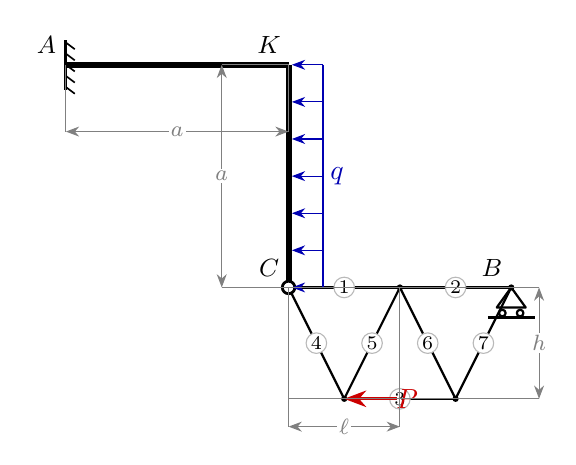
\begin{tikzpicture}[scale=0.707,>=Stealth,line join=round]
  \coordinate (P0) at (0.000,0.000);
  \coordinate (K) at (4.000,0.000);
  \coordinate (C) at (4.000,-4.000);
  \coordinate (TO1) at (6.000,-4.000);
  \coordinate (TO2) at (8.000,-4.000);
  \coordinate (TU0) at (5.000,-6.000);
  \coordinate (TU1) at (7.000,-6.000);
  \draw[thick] (C) -- (TO1);
  \draw[thick] (TO1) -- (TO2);
  \draw[thick] (TU0) -- (TU1);
  \draw[thick] (C) -- (TU0);
  \draw[thick] (TU0) -- (TO1);
  \draw[thick] (TO1) -- (TU1);
  \draw[thick] (TU1) -- (TO2);
  \draw[line width=2.2pt] (P0) -- (K);
  \draw[line width=2.2pt] (K) -- (C);
  \fill (TO1) circle (1.6pt);
  \fill (TO2) circle (1.6pt);
  \fill (TU0) circle (1.6pt);
  \fill (TU1) circle (1.6pt);
  \draw[fill=white,line width=1pt] (C) circle (3.2pt);
  \draw[line width=1.1pt] (0.000,-0.450) -- (0.000,0.450);
  \draw[line width=0.6pt] (0.000,-0.400) -- (0.160,-0.520);
  \draw[line width=0.6pt] (0.000,-0.200) -- (0.160,-0.320);
  \draw[line width=0.6pt] (0.000,0.000) -- (0.160,-0.120);
  \draw[line width=0.6pt] (0.000,0.200) -- (0.160,0.080);
  \draw[line width=0.6pt] (0.000,0.400) -- (0.160,0.280);
  \draw[thick] (8.000,-4.000) -- (7.740,-4.360) -- (8.260,-4.360) -- cycle;
  \draw[thick] (7.840,-4.460) circle (0.06) (8.160,-4.460) circle (0.06);
  \draw[line width=1pt] (7.580,-4.540) -- (8.420,-4.540);
  \node[circle,fill=white,draw=gray!55,inner sep=0.5pt,font=\scriptsize] at (5.000,-4.000) {1};
  \node[circle,fill=white,draw=gray!55,inner sep=0.5pt,font=\scriptsize] at (7.000,-4.000) {2};
  \node[circle,fill=white,draw=gray!55,inner sep=0.5pt,font=\scriptsize] at (6.000,-6.000) {3};
  \node[circle,fill=white,draw=gray!55,inner sep=0.5pt,font=\scriptsize] at (4.500,-5.000) {4};
  \node[circle,fill=white,draw=gray!55,inner sep=0.5pt,font=\scriptsize] at (5.500,-5.000) {5};
  \node[circle,fill=white,draw=gray!55,inner sep=0.5pt,font=\scriptsize] at (6.500,-5.000) {6};
  \node[circle,fill=white,draw=gray!55,inner sep=0.5pt,font=\scriptsize] at (7.500,-5.000) {7};
  \draw[->,blue!70!black] (4.620,0.000) -- (4.060,0.000);
  \draw[->,blue!70!black] (4.620,-0.667) -- (4.060,-0.667);
  \draw[->,blue!70!black] (4.620,-1.333) -- (4.060,-1.333);
  \draw[->,blue!70!black] (4.620,-2.000) -- (4.060,-2.000);
  \draw[->,blue!70!black] (4.620,-2.667) -- (4.060,-2.667);
  \draw[->,blue!70!black] (4.620,-3.333) -- (4.060,-3.333);
  \draw[->,blue!70!black] (4.620,-4.000) -- (4.060,-4.000);
  \draw[blue!70!black,thick] (4.620,0.000) -- (4.620,-4.000);
  \node[blue!70!black] at (4.870,-2.000) {$q$};
  \draw[->,red!80!black,line width=1.1pt] (5.950,-6.000) -- (5.000,-6.000);
  \node[red!80!black] at (6.130,-6.000) {$P$};
  \draw[thin,gray] (0.000,0.000) -- (0.000,-1.200);
  \draw[thin,gray] (4.000,0.000) -- (4.000,-1.200);
  \draw[<->,gray] (0.000,-1.200) -- (4.000,-1.200) node[midway,fill=white,inner sep=0.8pt,font=\footnotesize]{$a$};
  \draw[thin,gray] (4.000,0.000) -- (2.800,0.000);
  \draw[thin,gray] (4.000,-4.000) -- (2.800,-4.000);
  \draw[<->,gray] (2.800,0.000) -- (2.800,-4.000) node[midway,fill=white,inner sep=0.8pt,font=\footnotesize]{$a$};
  \draw[thin,gray] (4.000,-4.000) -- (4.000,-6.500);
  \draw[thin,gray] (6.000,-4.000) -- (6.000,-6.500);
  \draw[<->,gray] (4.000,-6.500) -- (6.000,-6.500) node[midway,fill=white,inner sep=0.8pt,font=\footnotesize]{$\ell$};
  \draw[thin,gray] (4.000,-4.000) -- (8.500,-4.000);
  \draw[thin,gray] (4.000,-6.000) -- (8.500,-6.000);
  \draw[<->,gray] (8.500,-4.000) -- (8.500,-6.000) node[midway,fill=white,inner sep=0.8pt,font=\footnotesize]{$h$};
  \node[font=\small] at (0.000,0.000) [xshift=-7pt,yshift=7pt] {$A$};
  \node[font=\small] at (4.000,0.000) [xshift=-7pt,yshift=7pt] {$K$};
  \node[font=\small] at (4.000,-4.000) [xshift=-7pt,yshift=7pt] {$C$};
  \node[font=\small] at (8.000,-4.000) [xshift=-7pt,yshift=7pt] {$B$};
\end{tikzpicture}
\end{center}
\textbf{Given quantities:}\quad $a=4$\,m\quad $\ell=2$\,m\quad $h=2$\,m\quad $q=2$\,kN/m\quad $P=15$\,kN
\par\medskip
\textbf{Tasks}\par
\begin{enumerate}[label=\textbf{\arabic*.}]
  \item Determine the degree of static determinacy.
  \item Compute all support reactions and hinge forces.
  \item Determine all truss member forces (tension/compression).
  \item Draw the section forces $N$, $V$, $M$ of the bending beams.
\end{enumerate}
\end{document}